\documentclass[12pt,a4paper]{article}
\usepackage[utf8]{inputenc}
\usepackage[spanish]{babel}
\usepackage{amsmath}
\usepackage{amsfonts}
\usepackage{amssymb}
\usepackage{graphicx}
\usepackage[left=2.5cm,right=2.5cm,top=3cm,bottom=3cm]{geometry}
\usepackage{xcolor}
\usepackage{listings}
\usepackage{tcolorbox}
\usepackage{hyperref}

% Configuración de colores para código
\definecolor{codegreen}{rgb}{0,0.6,0}
\definecolor{codegray}{rgb}{0.5,0.5,0.5}
\definecolor{codepurple}{rgb}{0.58,0,0.82}
\definecolor{backcolour}{rgb}{0.95,0.95,0.92}

\lstdefinestyle{mystyle}{
    backgroundcolor=\color{backcolour},   
    commentstyle=\color{codegreen},
    keywordstyle=\color{magenta},
    numberstyle=\tiny\color{codegray},
    stringstyle=\color{codepurple},
    basicstyle=\ttfamily\footnotesize,
    breakatwhitespace=false,         
    breaklines=true,                 
    captionpos=b,                    
    keepspaces=true,                 
    numbers=left,                    
    numbersep=5pt,                  
    showspaces=false,                
    showstringspaces=false,
    showtabs=false,                  
    tabsize=2
}
\lstset{style=mystyle}

\title{\textbf{Guía de Laboratorio 1}\\ \Large Servidor Web IoT con ESP32}
\author{Andrés Jaramillo - Andrea Zapata - Víctor Gonzales - Sergio Carmona - Daniela Nieto}
\date{\today}

\begin{document}

\maketitle

\section{Introducción}
En este proyecto se transforma un ESP32 en un poderoso Servidor Web Local para el Internet de las Cosas (IoT). Se vincula el mundo físico con el digital: usando un potenciómetro real para recopilar datos de voltaje y verlos graficados profesionalmente (con Google Charts y Plotly) en tiempo real en el navegador. Al mismo tiempo, se controla un LED físico de forma inalámbrica mediante una red Wi-Fi.

\section{Materiales y Ensamblaje del Circuito}
\begin{itemize}
    \item Placa ESP32 (DOIT ESP32 DEVKIT V1)
    \item Potenciómetro de $10\text{k}\Omega$
    \item LED y Resistencia ($220\Omega - 330\Omega$)
    \item Protoboard y Jumpers
\end{itemize}

\begin{tcolorbox}[colback=blue!5!white,colframe=blue!75!black,title=Detalle de Pines]
\textbf{Potenciómetro:} GND, GPIO34 (Señal), 3.3V.\\
\textbf{LED:} GPIO4 al Ánodo (mediante resistencia); GND al Cátodo.
\end{tcolorbox}

\begin{figure}[h]
    \centering
    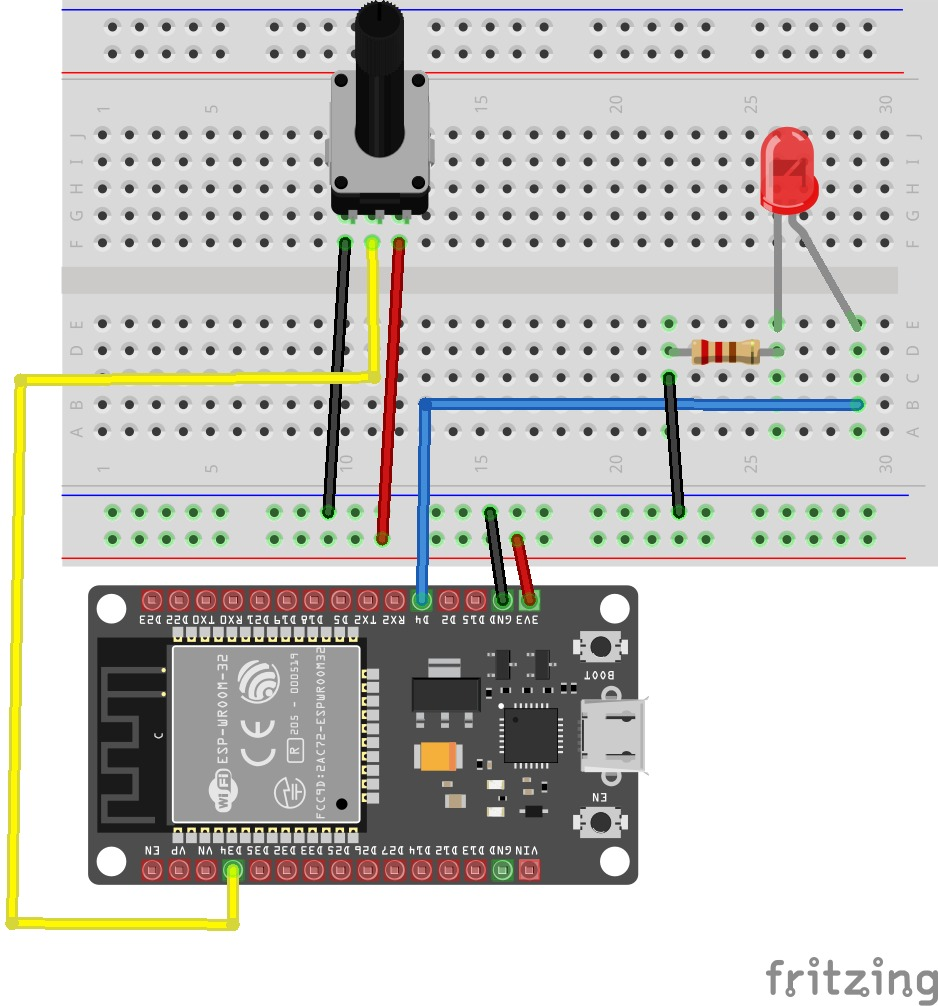
\includegraphics[width=0.7\textwidth]{circuito.jpeg}
    \caption{Diagrama de conexiones en la protoboard.}
\end{figure}

\subsection{Fotos del Ensamblaje Real}
\begin{figure}[h]
    \centering
    \begin{minipage}{0.32\textwidth}
        \centering
        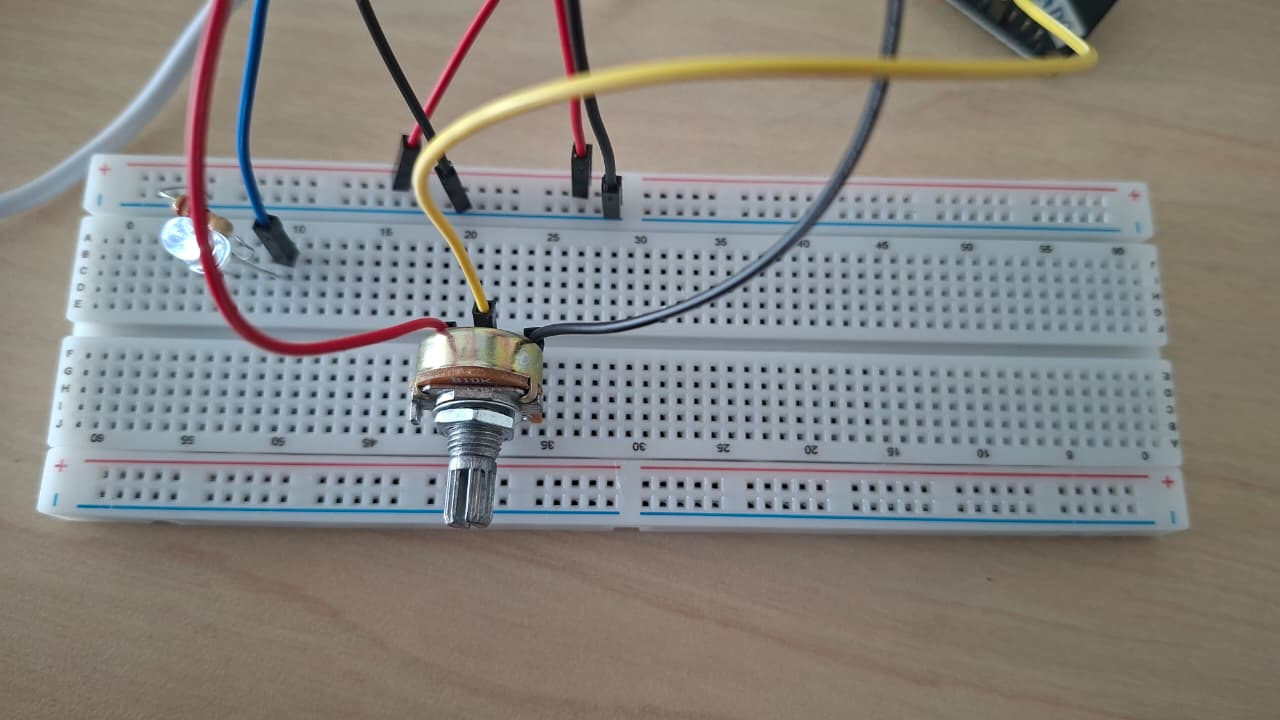
\includegraphics[width=\textwidth]{foto1.jpeg}
        \caption{Vista lateral.}
    \end{minipage}
    \hfill
    \begin{minipage}{0.32\textwidth}
        \centering
        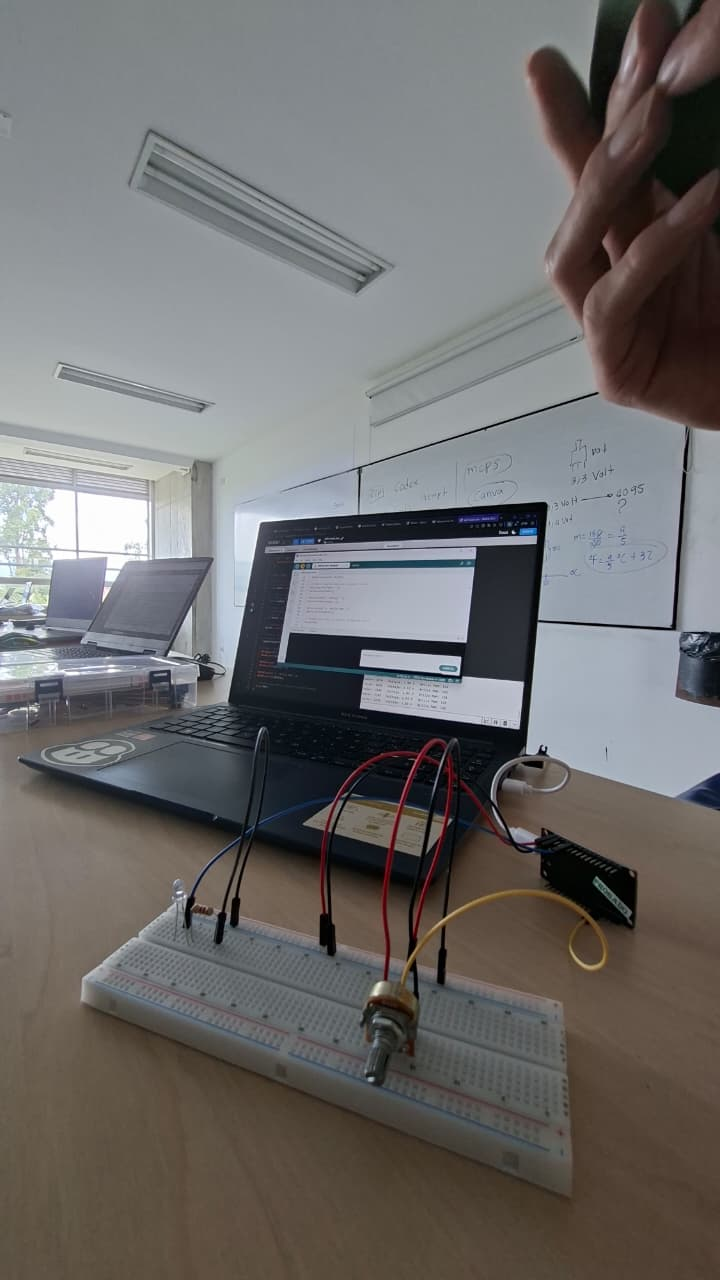
\includegraphics[width=\textwidth]{foto2.jpeg}
        \caption{Conexiones LED.}
    \end{minipage}
    \hfill
    \begin{minipage}{0.32\textwidth}
        \centering
        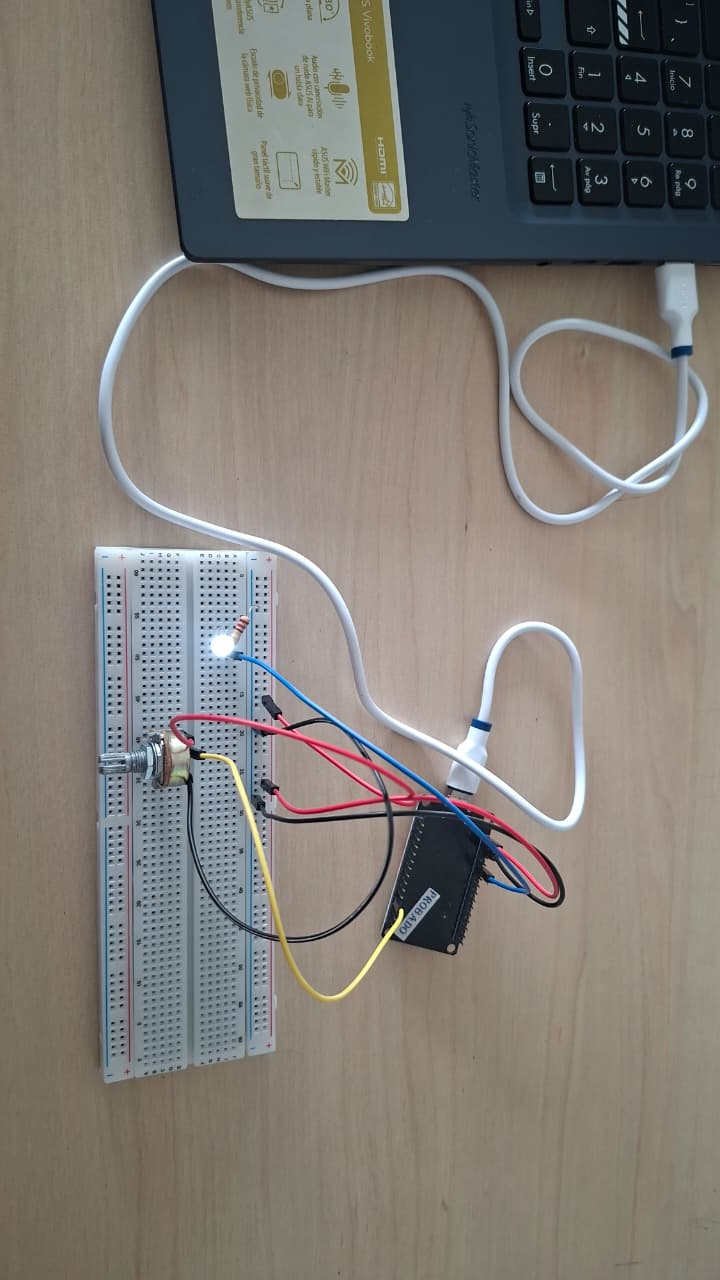
\includegraphics[width=\textwidth]{foto3.jpeg}
        \caption{Potenciómetro.}
    \end{minipage}
\end{figure}

\section{Código Fuente (Arduino IDE)}
\begin{lstlisting}[language=C++]
#include <WiFi.h>
#include <WebServer.h>

const char* miSSID     = "Andres";       
const char* miPASSWORD = "andres10";     

const int pinPotenciometro = 34; 
const int pinLED = 4;            

bool ledEncendido = false;
WebServer servidor(80);

void setup() {
  Serial.begin(115200);
  pinMode(pinLED, OUTPUT);
  digitalWrite(pinLED, LOW);

  WiFi.begin(miSSID, miPASSWORD);
  while (WiFi.status() != WL_CONNECTED) { 
      delay(500); 
      Serial.print("."); 
  }
  
  servidor.on("/", []() {
      // Aqui va el codigo HTML inyectado (ver archivo original)
      servidor.send(200, "text/html", "<h1>ESP32 Panel Activo</h1>");
  });

  servidor.on("/datos", []() {
    float v = (analogRead(pinPotenciometro) * 3.3) / 4095.0;
    servidor.send(200, "application/json", "{\"voltaje\": " + String(v, 2) + "}");
  });
  
  servidor.on("/led", []() {
    ledEncendido = !ledEncendido;
    digitalWrite(pinLED, ledEncendido ? HIGH : LOW);
    servidor.send(200, "text/plain", "OK");
  });

  servidor.begin();
}

void loop() { 
    servidor.handleClient(); 
}
\end{lstlisting}

\section{Instrucciones de Uso y Resultados}
\begin{enumerate}
    \item Configura tus credenciales de WiFi en el código.
    \item Sube el programa a la placa ESP32.
    \item Abre el Monitor Serie para obtener la dirección IP asignada.
    \begin{figure}[h]
        \centering
        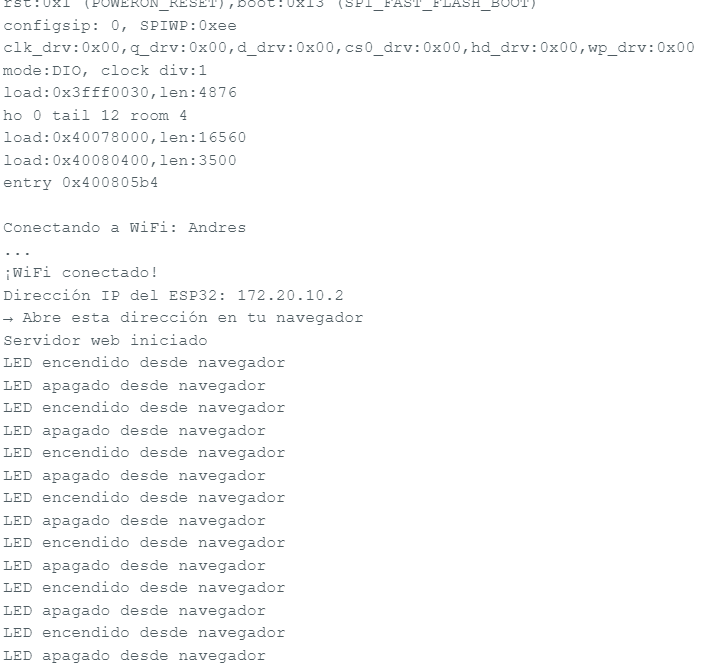
\includegraphics[width=0.8\textwidth]{terminal.png}
        \caption{Monitor Serie mostrando la dirección IP local.}
    \end{figure}
    \item Ingresa la IP en tu navegador para abrir el panel de control.
    \begin{figure}[h]
        \centering
        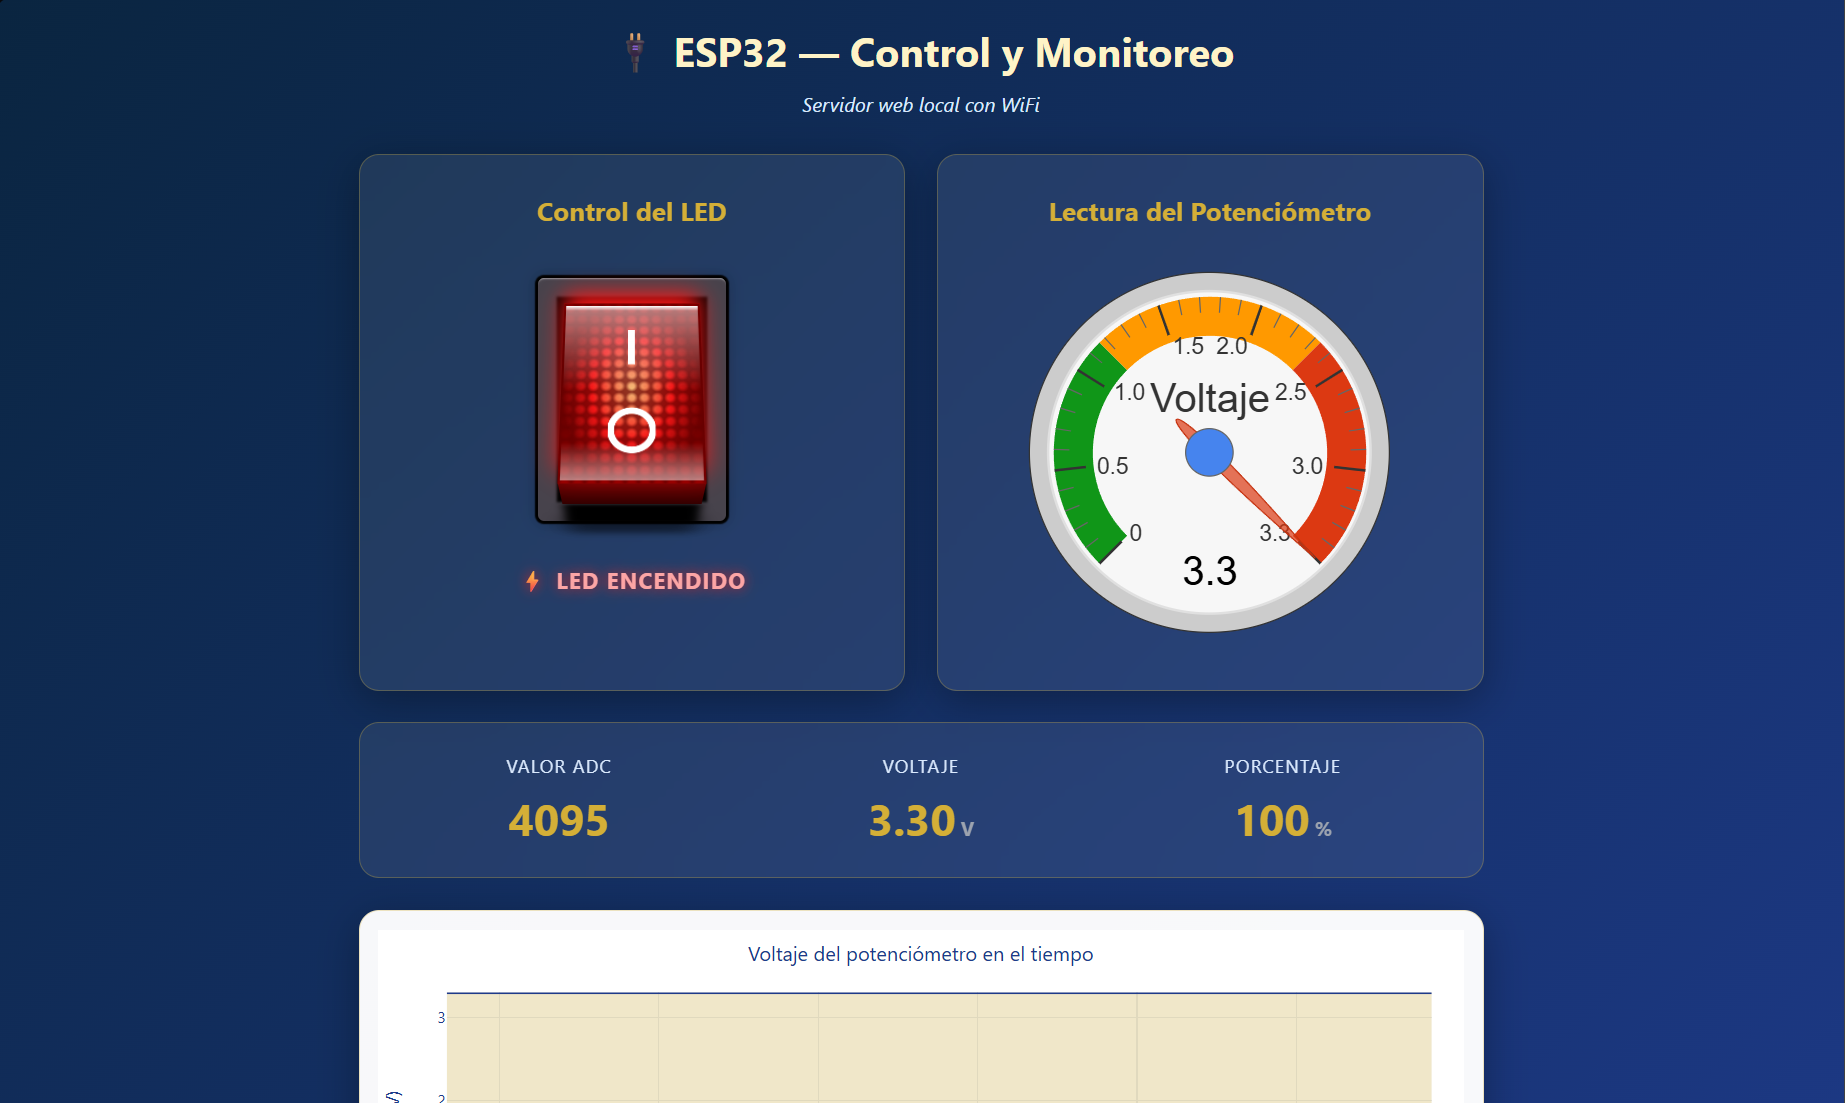
\includegraphics[width=0.8\textwidth]{paginaweb.png}
        \caption{Interfaz web interactiva con gráficas en tiempo real.}
    \end{figure}
\end{enumerate}

\end{document}
